% Created 2021-01-24 Sun 22:50
% Intended LaTeX compiler: pdflatex
\documentclass[11pt]{article}
\usepackage[utf8]{inputenc}
\usepackage[T1]{fontenc}
\usepackage{graphicx}
\usepackage{grffile}
\usepackage{longtable}
\usepackage{wrapfig}
\usepackage{rotating}
\usepackage[normalem]{ulem}
\usepackage{amsmath}
\usepackage{textcomp}
\usepackage{amssymb}
\usepackage{capt-of}
\usepackage{hyperref}
\usepackage{minted}
\hypersetup{colorlinks=true, linkcolor=black, filecolor=red, urlcolor=blue}
\usepackage[turkish]{babel}
\author{Eren Hatırnaz}
\date{21 Temmuz 2019}
\title{Yazılım Gündemi - 2\\\medskip
\large 15-21 Temmuz 2019}
\hypersetup{
 pdfauthor={Eren Hatırnaz},
 pdftitle={Yazılım Gündemi - 2},
 pdfkeywords={},
 pdfsubject={},
 pdfcreator={Emacs 27.1 (Org mode 9.3)},
 pdflang={Turkish}}
\begin{document}

\maketitle
\tableofcontents \clearpage\shorthandoff{=}

\begin{center}
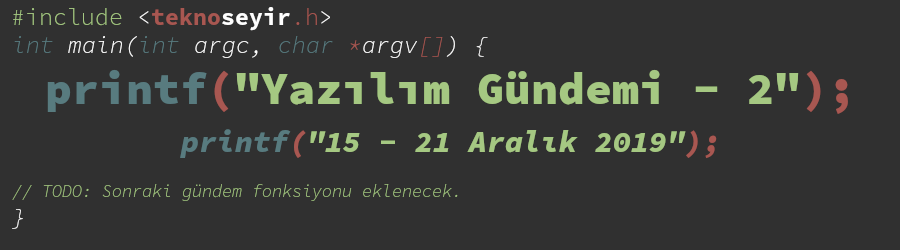
\includegraphics[width=.9\linewidth]{gorseller/yazilim-gundemi-banner.png}
\end{center}

\begin{center}
\href{../01/yazilim-gundemi-01.pdf}{< Önceki Gündem} | \textbf{15-21 Temmuz 2019} | \href{../03/yazilim-gundemi-03.pdf}{Sonraki Gündem >}

\href{https://teknoseyir.com/blog/yazilim-gundemi-2-15-21-temmuz-2019}{TeknoSeyir'de Oku}
\end{center}

\section{GNU/Linux sunucuları hedef alan 3 zararlı Python kütüphanesi \href{https://www.zdnet.com/article/malicious-python-libraries-targeting-linux-servers-removed-from-pypi/}{PyPI üzerinden silindi}}
\label{sec:org1ab69f7}
ReversingLabs isimli güvenlik firması, PyPI (Python Package Index) üzerinde
neredeyse 20 aydır (Kasım 2017'den beri) bulunan ve sadece GNU/Linux sistemlere
kurulduğunda aktif olan zararlı kod parçaları içeren 3 kütüphaneyi tespit etti.
\textbf{ruri12} kullanıcı adı altında yayınlanmış bu üç kütüphanenin isimleri şunlar:
\textbf{libpeshnx}, \textbf{libpesh} ve \textbf{libari}. Üzerinde çalıştığınız ya da bağımlılık
olarak projenize eklediğiniz kütüphanelerde bu paket isimleri var mı diye
bakmanız iyi olacaktır.

\begin{figure}[htbp]
\centering
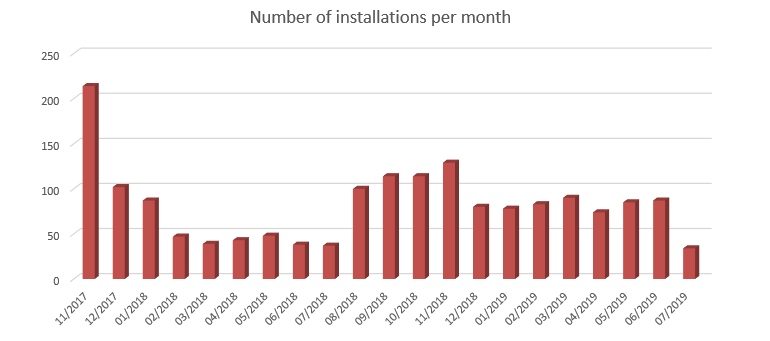
\includegraphics[width=.9\linewidth]{gorseller/zararli-kutuphane-pypi.png}
\caption{Zararlı kütüphanenin aylara göre indirilme sayıları}
\end{figure}

Kullanıcı tarafından çalıştırılınca sisteme uzaktan komut göndermeye olanak
sağlayan bu arka kapı sadece \texttt{libpeshnx} isimli kütüphanede olsa da, diğer 2
kütüphanenin de zararlı kod parçaları içerdiği tespit edilmiş.

Güvenlik firmasının uyarısı üzerine bu 3 pakette PyPI sistemi üzerinden
silinmişler. İncelemek için kaynak kodlarını bulmaya çalıştım fakat bulamadım.
Geçtiğimiz hafta da buna benzer "kütüphanede arka kapı bulundu" haberi vardı,
görünen o ki bu tarz haberler çıkmaya devam edecek ve artık umarım geliştirici
camiası olarak bazı şeyleri sorgulamaya başlamamıza vesile olacak.
\section{Python 3.8 ile gelecek olan \href{https://www.python.org/dev/peps/pep-0569/\#features-for-3-8}{yeni özellikler belli oldu}}
\label{sec:org23c783a}
Python 3.8.0 Beta 1 sürümü 4 Haziran'da \href{https://www.python.org/downloads/release/python-380b1/}{yayınlanmıştı}. Beta 2 sürümü de 4
Temmuz'da \href{https://www.python.org/downloads/release/python-380b2/}{yayınlandı}. \href{https://www.python.org/dev/peps/pep-0569/\#release-schedule}{Plan dokümanı}nda belirttiklerine göre Beta 1'den sonra
yeni özellik (feature) eklenmeyecek, hata gidermeleri ve iyileştirmelere
odaklanılacak. Önümüzdeki aylarda da Beta süreci devam edecek ve ardından ilk
Release Candidate sürümünün 30 Eylül'de, final sürümünün ise 21 Ekim'de
duyurulması bekleniyor. İlgimi çeken özellikleri inceledim, diğerlerini de siz
inceleyebilirsiniz.
\subsection{':=' Walrus Operatörü (\href{https://www.python.org/dev/peps/pep-0572/}{PEP572 - Assignment Expressions})}
\label{sec:org9c7e524}
\begin{figure}[htbp]
\centering
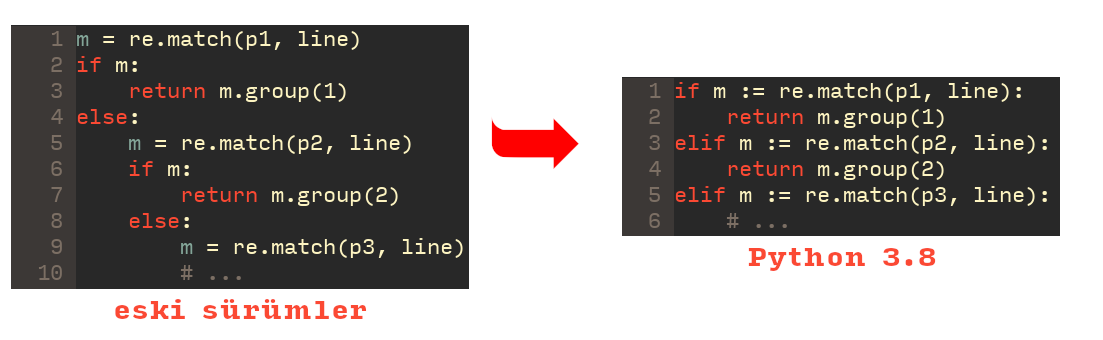
\includegraphics[width=.9\linewidth]{gorseller/python38-walrus-fixed.png}
\caption{Python 3.8 ile birlikte gelecek olan walrus operatorü}
\end{figure}

Yukarıdaki örnekte de görüldüğü gibi, bu yeni operator sayesinde, önceden
\texttt{if} sorgusunda kullanacağımız değişkeni tanımlamamız gerekirken artık direkt
\texttt{if} sorgusu içerisinde tanımlayıp, if'in içerisinde kullanabileceğiz. Benim
de zaman zaman eksikliğini hissettiğim bir özellikti, gelmesine sevindim.
\subsection{Sadece pozisyonel parametreler (\href{https://www.python.org/dev/peps/pep-0570/}{PEP 570 - Positional-Only Parameters})}
\label{sec:org150f7bc}
Python'da bir fonksiyona parametre gönderirken ille de sırayla göndermek
zorunda değiliz. Mesela \texttt{def merhaba(isim, mesaj)} diye bir fonksiyon varsa
bu şekilde de parametre gönderebiliyoruz: \texttt{merhaba(mesaj=deneme, isim=eren)}.
Fakat artık eğer istenirse sadece pozisyonel parametreler de
tanımlanabilecek. Çok sık Python yazmadığım için tam olarak hangi sorunu
çözüyor bilemiyorum ama eklendiğine göre ihtiyaç vardı demekki. Detaylı bilgi
için mutlaka PEP sayfasına bakın. Özellikle "How To Teach This" başlığı
altındaki kısıma bakmanızı tavsiye ederim. Sadece özelliği geliştirip
bırakmamışlar, aynı zamanda bunun insanlara nasıl öğretileceğini de
açıklamışlar.

Diğer yenilikler için \href{https://www.python.org/dev/peps/pep-0569/\#features-for-3-8}{bu PEP sayfasını ziyaret} edebilirsiniz.
\section{C++20 için komite taslağı \href{https://www.reddit.com/r/cpp/comments/cfk9de/201907\_cologne\_iso\_c\_committee\_trip\_report\_the/}{hazırlanmış}}
\label{sec:org373ef23}
Bildiğiniz gibi C++ programlama dilinin her 3 yılda bir yeni sürümü çıkıyor.
Önümüzdeki yıl çıkacak olan C++20 için de ISO C++ Komitesi toplanmış ve yeni
eklenecek olan özelliklere karar vermişler. C++ diline hiç hakim olmadığım için
yeni eklenecek özellileri de pek inceleyemedim fakat bağlantısını verdiğin
reddit gönderisinde liste halinde yeni özellikleri ve diğer bilgileri
bulabilirsiniz. C++20'nin 2020 ilkbaharında yayınlanması bekleniyor.
\subsection{\href{http://www.open-std.org/jtc1/sc22/wg21/docs/papers/2019/p0645r9.html}{std::format} ile metin biçimlendirme}
\label{sec:org103d0b6}
Diğer birçok programlama dilinde de karşılaştığımız string içerisinde değişken
kullanmaya olanak sağlayan özellik C++20'de geliyor. Örnek vermek gerekirse:

Eskiden bu şekilde yazdığımız satır:

\begin{minted}[breaklines=true,breakanywhere=true,frame=lines, linenos, label=C++, labelposition=topline]{cpp}
cout << "Merhaba, " << kullanici_adi << ".\n";
cout << "Toplam " << okunmamis_mesaj_sayisi << " adet okunmamış mesajınız var!\n";
\end{minted}

Artık bu şekilde sadeleşecek:
\begin{minted}[breaklines=true,breakanywhere=true,frame=lines, linenos, label=C++, labelposition=topline]{cpp}
std::format("Merhaba, {}.\n", kullanici_adi);
std::format("Toplam {} adet okunmamış mesajınız var!\n", okunmamis_mesaj_sayisi);
\end{minted}
\section{Go geliştiricileri, dilin içerisine hata kontrol fonksiyonu ekleme isteğini reddetti}
\label{sec:orgdd9f5e1}
5 Haziran'dan beri Github üzerinde tartışılan bu konu, 17 Temmuz'da issue
sayfasını açan takım üyesinin \href{https://github.com/golang/go/issues/32437\#issuecomment-512035919}{yazdığı yorum} ile reddedildiği duyuruldu. Diğer
programlama dillerinde \texttt{try \{\} catch () \{\}} gibi söz dizimleri ile sıkça
gördüğümüz özellik Go dilinde henüz mevcut değil. Şu an şöyle bir yapı
kullanılıyor:

\begin{minted}[breaklines=true,breakanywhere=true,frame=lines, linenos, label=Go, labelposition=topline]{go}
f, err := os.Open(filename)

if err != nil {
  return …, err
}
\end{minted}

Bu kullanımdaki sorun 2018'de Russ Cox tarafından \href{https://go.googlesource.com/proposal/+/master/design/go2draft-error-handling-overview.md}{detaylıca raporlanmıştı}.
Özetlemek gerekirse, yukarıdaki kullanım kod karmaşıklığını arttırdığı gibi
kodun temiz görünmesinin de önüne geçiyor, iddiası var. Raporda taslak olarak
bir çözüm önerilmiş fakat sonuç olarak 2019 Haziran'da \texttt{try} fonksiyonu \href{https://github.com/golang/proposal/blob/master/design/32437-try-builtin.md}{tasarı
olarak yazılmış} ve bugün konuşulan bu halini almış:

\begin{minted}[breaklines=true,breakanywhere=true,frame=lines, linenos, label=Go, labelposition=topline]{go}
f := try(os.Open(filename))
\end{minted}

Görüldüğü gibi yukarıdaki yapıdan daha sade ve temiz bir hata yakalama olanağı
sunuyor. Burada şunu belirtmekte fayda var: Dile yeni bir anahtar kelime
(keyword) eklenmeyecek, yeni bir fonksiyon olarak eklenecek bu özellik.
Github'daki tartışma çok uzun, yüzlerce yorum yazılmış hepsini okuyamadım fakat
issue yazarının hazırladığı tartışma özetlerini(1 2) okudum, tüm tartışmayı
okuyamadığım ve dile de pek hakim olmadığım için yorum yapamayacağım fakat
sonuç olarak bu istek reddedilmiş. Anladığım kadarıyla pek sağlıklı bir
tartışma ortamı da kurulamamış gözüküyor.
\section{MSRC organizasyonu güvenli programlama dillerini \href{https://www.zdnet.com/article/microsoft-to-explore-using-rust/}{keşfetmeye Rust ile başladı}}
\label{sec:org22b39ed}
Microsoft Security Response Centre organizasyonu, bloglarında bu hafta
yayınladıkları \href{https://msrc-blog.microsoft.com/2019/07/16/a-proactive-approach-to-more-secure-code/}{blog yazısı} ile birlikte yeni bir yazı serisine başladıklarını
duyurdu. Bu yazı serisinin amacı güvenli programlama dillerini keşfetmek ve
incelemek olacakmış. Mozilla tarafından geliştirilen, son zamanlarda özellikle
bellek-korumalı (memory-safe) yapısı nedeniyle popülaritesi artan \href{https://www.rust-lang.org/}{Rust}
programlama dilini de bu yazı serisi için başlangıç olarak seçmişler.
Çalışmalarını takip etmeye çalışacağım.
\section{ABD Finansal Hizmetler Komitesi'nde \href{https://www.c-span.org/video/?c4808083/rust-language-chosen}{Rust konuşuldu}}
\label{sec:orgb4e68ad}
Komitenin toplanma nedenini tam olarak bilmiyorum fakat Facebook'un
geliştirdiği kripto para Libra hakkında olduğu açıkça belli. Komite üyesi,
Facebook'dan yetkili olduğunu düşündüğüm kişiye "\href{https://github.com/libra/libra}{GitHub deponuza} baktım
projenin büyük bir bölümü Rust dilini kullanıyor. Rust neden seçildi? Rust
dilinin güvenlik sorunları için yeterli olduğuna inanıyor musunuz?" şeklinde
bir soru sordu. Facebook yetkilisinin verdiği cevaptan sonra komite üyesi, bu
sefer de "Libra, Rust dilinin Nightly Build (stabil olmayan) sürümünü
kullanıyor. Nightly Build sürümde tam olarak hangi özelliklere ihtiyacınız var
ve neden stabil sürümleri kullanmıyorsunuz?" şeklinde bir soru soruyor. Bir
bürokratın bu konulara bu kadar hakim olması beni şaşırttı. Bizdeki "\href{https://www.youtube.com/watch?v=Sn7pNTsY5iY}{bulut
bilişim}" vakası akıllara gelince insan imreniyor tabi\ldots{}
\section{JDK 13 sürümü "Rampdown" \href{https://mail.openjdk.java.net/pipermail/jdk-dev/2019-July/003170.html}{ikinci aşamaya geçti}}
\label{sec:orgc502bd4}
OpenJDK takımı 13 sürümü için yeni özellik (feature) seti kabul etmeyi
durdurdu. Bu aşamadan sonra yeni özellik eklemek yerine \href{https://bugs.openjdk.java.net/browse/JDK-8226964?filter=33405}{raporlanan hataları}
gidermeye odaklanacaklarmış. \href{http://openjdk.java.net/projects/jdk/13/\#Schedule}{Planladıkları takvimine göre} ilk RC (Release
Candidate) sürümü 8 Ağustos, final RC sürümü ise 22 Ağustos tarihinde
yayınlanacak gibi gözüküyor. Sürümün genel kullanılabilirlik durumuna gelmesi
de 17 Eylül tarihini bulacak.
\newpage
\section{Google, açık bulanlara verilen \href{https://security.googleblog.com/2019/07/bigger-rewards-for-security-bugs.html}{ödül miktarlarını arttırdı}}
\label{sec:org93f2c6e}
Yeni ödül tablosu bu şekilde:

\begin{figure}[htbp]
\centering
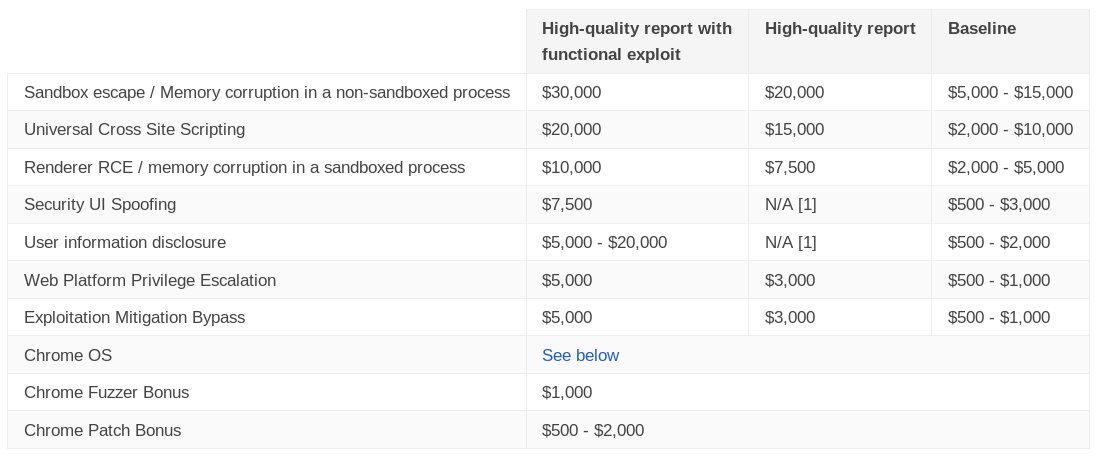
\includegraphics[width=.9\linewidth]{gorseller/google-odulleri-arttirdi.png}
\caption[//www.google.com/about/appsecurity/chrome-rewards/index.html\#rewards]{Tablo kaynağı: \url{https://www.google.com/about/appsecurity/chrome-rewards/index.html\#rewards}}
\end{figure}

Hadi bakalım klavyeler çalışsın! :)
\section{Diğer Haberler}
\label{sec:org89173a3}
\begin{itemize}
\item Yazılım üzerine yeni bir türkçe podcast serisi başladı: \href{https://kodpod.live/}{kodpod}.
\item NIST, Amerika'da Yapay Zeka Standartları belirlemeye çalışıyor. \href{https://www.nist.gov/sites/default/files/documents/2019/07/02/plan\_for\_ai\_standards\_publicreview\_2july2019.pdf}{Taslak Metin}
\item TypeScript 3.6 Beta \href{https://devblogs.microsoft.com/typescript/announcing-typescript-3-6-beta/}{duyuruldu}
\item Nim programlama dilinin 0.20.2 sürümü \href{https://nim-lang.org/blog/2019/07/17/version-0202-released.html}{yayınlandı}.
\item Google, Chrome içersinden XSS Auditor aracını \href{https://nakedsecurity.sophos.com/2019/07/18/google-chrome-is-ditching-its-xss-detection-tool/}{kaldırıyor}.
\item Küçük boyutuyla öne çıkan Go derleyicisinin 0.7.0 sürümü \href{https://github.com/tinygo-org/tinygo/releases/tag/v0.7.0}{duyuruldu}.
\item Volta JavaScript Launcher v0.5.7 sürümü \href{https://github.com/volta-cli/volta/releases/tag/v0.5.7}{duyuruldu}.
\item JavaScript ve TypeScript'de GraphQL için otomatik tamamlama özelliği sunan
araç açık kaynak olarak yayınlandı: \href{https://github.com/graphql-editor/graphql-zeus}{graphql-zeus}.
\item Birden fazla veritabanını tek bir SQL sorgusunda kullanmaya olanak sağlayan
araç açık kaynak olarak yayınlandı: \href{https://github.com/cube2222/octosql}{octosql}
\item YugaByte DB ürünü \href{https://blog.yugabyte.com/why-we-changed-yugabyte-db-licensing-to-100-open-source/}{açık kaynak oldu}. \href{https://github.com/YugaByte/yugabyte-db}{GitHub Deposu}
\item Zstandard 1.4.1 sürümü \href{https://github.com/facebook/zstd/releases/tag/v1.4.1}{duyuruldu}.
\item Dağıtık işlemsel anahtar-değer (key-value) veritabanı TiKV 3.0 sürümü
\href{https://tikv.org/blog/tikv-3.0ga/}{duyuruldu}. \href{https://github.com/tikv/tikv}{GitHub Deposu}
\item Dağıtık yapay zeka projeleri için TensorFlow kütüphanesi yayınlandı: \href{https://github.com/zurutech/ashpy}{ashpy}.
\item Microservisler için komut satırı aracı monday 0.0.9 sürümü \href{https://github.com/eko/monday/releases/tag/0.0.9}{duyuruldu}.
\item Rust uygulamaları için güvenlik odaklı uygulama framework sisteminin v0.2.0
sürümü yayınlandı: \href{https://iqlusion.blog/introducing-abscissa-rust-application-framework}{abscissa}. \href{https://github.com/iqlusioninc/abscissa}{GitHub Deposu}
\item Veritabanı yönetim aracı ElectroCRUD 2.2.0 beta sürümü \href{https://github.com/garrylachman/ElectroCRUD/releases/tag/2.2.0-beta}{duyuruldu}.
\item Akademik yayınlar:
\begin{itemize}
\item \href{https://arxiv.org/abs/1907.07804}{OmniNet: A unified architecture for multi-modal multi-task learning} Github
deposu: \url{https://github.com/subho406/OmniNet}
\item \href{https://arxiv.org/abs/1907.07587}{A Differentiable Programming System to Bridge Machine Learning and
Scientific Computing}
\item \href{https://arxiv.org/abs/1907.03890}{Manticore: A User-Friendly Symbolic Execution Framework for Binaries and
Smart Contracts}
\end{itemize}
\end{itemize}
\section{Lisans}
\label{sec:orgf92bc7b}
\begin{center}
\begin{center}

\includegraphics[height=1.5cm]{../../../img/CC_BY-NC-SA_4.0.png}
\end{center}

\href{yazilim-gundemi-02.pdf}{Yazılım Gündemi - 2} yazısı \href{https://erenhatirnaz.github.io}{Eren Hatırnaz} tarafından \href{http://creativecommons.org/licenses/by-nc-sa/4.0/}{Creative Commons
Atıf-GayriTicari-AynıLisanslaPaylaş 4.0 Uluslararası Lisansı} (CC BY-NC-SA 4.0)
ile lisanslanmıştır.
\end{center}
\end{document}
